\documentclass[11pt,letterpaper]{article}
\usepackage[margin=1in]{geometry}
\usepackage[T1]{fontenc}
\usepackage{lmodern,microtype,graphicx,booktabs,float}
\usepackage[hidelinks]{hyperref}
\setlength{\parindent}{0pt}
\setlength{\parskip}{3pt}
\pagestyle{empty}
\newcommand{\abstractsection}[1]{\par\vspace{3pt}\noindent\textbf{#1}\par\nobreak}
\author{Aaron John Danielson\textsuperscript{1,*}\quad Denis Beausoleil\quad Hasan Alanam\\
\textsuperscript{1}Department of Computer Science, The University of Texas at Austin\\
\textsuperscript{*}Corresponding author: \href{mailto:aaron.danielson@austin.utexas.edu}{aaron.danielson@austin.utexas.edu}}
\hypersetup{pdftitle={Future Proves Past: Learning Backward to Forecast International NCAA Recruits},pdfauthor={Aaron John Danielson, Denis Beausoleil, Hasan Alanam}}

\begin{document}
\begin{center}
{\large\bfseries Future Proves Past: Learning Backward\\
to Forecast International NCAA Recruits}
\par\vspace{5pt}
{\small\makeatletter\@author\makeatother}
\end{center}
\vspace{-10pt}

\abstractsection{Introduction}
International recruiting faces a complex challenge: how will a player's performance abroad translate to the NCAA? Programs must make that forecast before committing roster spots and NIL resources. The need for better methods is growing: in 2025--26, 113 entrants had substantial professional experience, versus fewer than 15 per season before 2022. Yet historical examples of the international-to-NCAA transition remain limited. Far more evidence lies in the reverse direction: more than 10,000 former NCAA players later competed abroad or for national teams, observed in both settings. We use these later careers as auxiliary supervision for a neural model whose shared parameters inform freshman forecasts. Building on league-translation research [1], we ask whether this additional evidence improves freshman forecasts and whether the gains extend to players without international or national-team experience.

\abstractsection{Methods}
From over six million player-game records (NCAA, 160 international leagues, national teams), our multitask deep learning model [2] learns to forecast NCAA seasons from earlier games and reconstruct known college seasons from later games. Both tasks share one network conditioned on age, time, competition and destination context. The former players' careers train the model that evaluates recruits. It predicts distributions over participation, playing time and production. Projected onto standardized player profiles, it yields NCAA-equivalent translation rules per statistic. The full model is paired with an identical control trained without post-NCAA data.

\abstractsection{Results}
On the holdout seasons, the statistics freshmen with international or national-team experience went on to produce are 2.3 to 5.8 times more probable under the full model, all 95\% intervals above one (Figure~\ref{fig:evidence}). The gain resides in production for players with nontrivial playing time; the largest improvements are breakout seasons the control missed (Figure~\ref{fig:cases}). On the 2025--26 test (two fits averaged), the seasons of the 307 freshmen with international, national-team or showcase games are 1.5 times more probable (interval 1.1--2.0) and the continuous ranked probability score improves by 6--8\% for season minutes, points, rebounds and assists. Freshmen without such history do not benefit. The model also ranks the test freshmen better than the 247Sports recruiting composite: rank correlation with season minutes 0.40--0.43 versus 0.23, and AUC for reaching 400 minutes 0.69--0.72 versus 0.61.

\abstractsection{Conclusion}
With millions in NIL dollars at stake, learning backward to forecast the future can mean the difference between a championship roster and recruiting mistakes that jeopardize a coach's job and a program's future.
% Learning from later careers improves freshman forecasts and gives programs a broader evidence base for international recruiting.

\vspace{0pt}
{\small
\textbf{References}\par
[1] Glazer, A.\ K.\ (2026). Nuthin' But A G League: Estimating league translation factors. \emph{Journal of Sports Analytics}. \href{https://doi.org/10.1177/22150218261428808}{doi:10.1177/22150218261428808}.\par
[2] Caruana, R.\ (1997). Multitask Learning. \emph{Machine Learning}, 28, 41--75. \href{https://doi.org/10.1023/A:1007379606734}{doi:10.1023/A:1007379606734}.\par
Code and documentation: \url{https://github.com/aaronjdanielson/future_proves_past}
}

\clearpage
\begin{figure}[H]
\centering
\includegraphics[width=\linewidth]{figures/fig_learning_and_evidence_crps_dark.pdf}
\caption{Cohorts with international or national-team history; two fits per season averaged.}
\label{fig:evidence}
\end{figure}

\begin{figure}[H]
\centering
\includegraphics[width=\linewidth]{figures/fig_case_distributions_dark.pdf}
\caption{The six 2025--26 test freshmen (20+ pre-college games, 400+ minutes) whose seasons gained most from later-career training; 2,000 simulated seasons per model; gold: actual season.}
\label{fig:cases}
\end{figure}

\end{document}
